\lecture{5}{16 Sep. 15:30}{}
We can observe that the number of ways of partitioning \(n\) distinct items into \(k\) distinct nonempty groups is \(S(n, k) k!\). 

\begin{question}
    How many ways can we partition \(n\) distinct items into \(l\) distinct groups (not necessarily nonempty)?
\end{question}
\begin{answer}
    \(l^n\): product rule, each element has \(l\) choice for which group to go to.   
\end{answer}
\begin{proof}[Alternative method]
    Count by the number of nonempty groups \((k)\), and then use sum rule. Partition elements into \(k\) nonempty indistinguishable groups, which has \(S(n, k)\) choices, and then map the \(k\) sets to the \(l\) groups injectively, so there are \(l^{\underline{k}} = l(l - 1) \dots (l - k + 1)\) choices. Hence, the total number of partition is 
    \[
        \sum_{k=0}^l S(n, k) l^{\underline{k}}.
    \]
        By double counting, we know 
    \[
        l^n = \sum_{k=0}^n S(n, k) l^{\underline{k}} = \sum_{k=0}^n S(n, k) l^{\underline{k}}. 
    \]     
\end{proof}
\begin{proposition} \label{prop: x^n is sum S(n,k)x^underline(k) is true for any field}
    For any field \(F\), and \(x \in F\), \(n \in \mathbb{N} \cup \left\{ 0 \right\} \), then 
    \[
        x^n = \sum_{k=0}^n S(n, k) x^{\underline{k}}. 
    \]   
    (We define \(x^{\underline{k}} = x(x-1) \dots (x - (k-1))\).)
\end{proposition}

\begin{proof}
    There are polynomials of degree \(\le n\) that agree for all \(x \in \mathbb{N} \), so they must agree everywhere.  
\end{proof}

We can observe that \(\left\{ x^n \mid n \in \mathbb{N} \cup \left\{ 0 \right\}  \right\} \) forms a basis for 
\[
    F[x] = \left\{ \sum_{k=0}^n a_k x^k : a_k \in F  \right\}. 
\] 
Since \(x^n\) is a linear combination of \(\left\{ x^{\underline{n}} \mid n \in \mathbb{N} \cup \left\{ 0 \right\}  \right\} \), that means this is also a basis for \(F[x]\). And the proposition shows that the change of basis matrix is the matrix of Stirling numbers of the second kind: 
\[
    \begin{pmatrix}
         1&  &  &  & 0 & 0  \\
         &  1&  &  &  & 0  \\
         &  &  1&  &  &   \\
         &  &  &  \ddots&  &   \\
         &  &  &  &  \ddots&   \\
         S(n, k)&  &  &  &  &1   \\
    \end{pmatrix}
    \begin{pmatrix}
         x^{\underline{0}} \\
         x^{\underline{1}}  \\
         x^{\underline{2}}  \\
         \vdots \\
          x^{\underline{k}} \\
          \vdots\\
    \end{pmatrix} = 
    \begin{pmatrix}
         x^0 \\
         x^1 \\
         x^2\\
          \vdots\\
          x^k\\
          \vdots\\
    \end{pmatrix}.
\]   
\section{Stirling numbers of the first kind}
    Recall the permutation \(\pi \) is a bijection from \([n]\) to \([n]\). 

\begin{eg}
    \(\pi = 32154\), then \(\pi (1) = 3, \pi (2) = 2, \pi (3) = 1, \pi (4) = 5, \pi (5) = 4\). 
\end{eg}

\begin{eg}
    \(\pi _1 = 312, \pi _2 = 213\), then \(\pi _2 \circ \pi _1 = 321\) and \(\pi _1 \circ \pi _2 = 132\).  
\end{eg}

\begin{claim}
    \(\forall \pi \in S_n\), \(\forall x \in [n]\), \(\exists i \in [n]\) s.t. \(\pi ^i (x) = x\).    
\end{claim}
\begin{proof}
    Consider \(\pi ^1(x), \pi ^2(x) ,\dots , \pi ^n(x) \in [n]\), if any are equal to \(x\), then we're done. Otherwise, there are only \(n - 1\) possible values, which are \([n]\setminus \left\{ x \right\} \). Hence, there are some \(j_1, j_2 \in [n]\) with \(j_1 > j_2\) and \(\pi ^{j_1}(x) = \pi ^{j_2}(x)\) by Pigeonhole principle. Applying \(\pi ^{-1}\) for \(j_2\) times, we get 
    \[
        \pi ^{j_1 - j_2}(x) = x \quad \text{with } 1 \le j_1 - j_2 \le n,
    \] which is a contradiction.
\end{proof}

\begin{definition}[cycle]
    For the smallest \(i\), \(1 \le i \le n\) with \(\pi ^i (x) =x\), we say 
    \[
        (x \ \pi (x) \ \pi ^2(x) \ \dots \ \pi ^{i-1}(x))
    \] is the cycle of \(x\).   
\end{definition}

It follows that every permutation is a union of disjoint cycles. Hence, we have cycle representation of \(\pi \). 

\begin{eg}
    \(\pi = 32154\), the cycle form is \((13)(2)(45)\).  
\end{eg}

\begin{definition}[fixed point and transposition]
    A fixed point of a permutation is a cycle of length \(1\) i.e. an element \(x\) with \(\pi (x) = x\). A transposition is a cycle of length \(2\). A permutation is cyclic if it has a single cycle (of length \(n\)).
\end{definition}

\begin{question}
    How many cyclic permutations of \([n]\) are there? 
\end{question}
\begin{answer}
    \((n-1)!\). We can first fix the head of the cycle to be \(1\), then for \(\pi (1)\), we have \(n-1\) choices, and for \(\pi ^2(1)\), we have \(n - 2\) choices, and so on, so we have \((n-1)!\) cyclic permutations. 
    \begin{note}
        Who is in the head of the cycle is not important.
    \end{note}     
\end{answer}

\begin{definition}[The Stirling numbers of the first kind] \label{def: Stirling number for the first kind}
    \(s_{n, k}\) (or \([s(n, k)]\)) enumerate the permutation in \(S_n\) with exactly \(k\) cycles.   
\end{definition}

\begin{eg}
    \(s_{n, 1} = (n-1)!, s_{n,n} = 1, s_{n, n-1} = \binom{n}{2}, s_{n, 2} =\)not so obvious.
\end{eg}
\begin{explanation}
    \begin{align*}
        s_{n, 2} &= \frac{1}{2}\sum_{k=1}^{n-1} \binom{n}{k}(k-1)!(n-k-1)! 
    \end{align*}
    Note that we multiply it by \(\frac{1}{2}\) since we count each cycle-pair twice. Also, we know that a cycle of length \(n\) has \((n-1)!\) choices if we fix all \(n\) members in the cycle.   
    
    Alternatively, say the "first" cycle is the one containing \(1\) together with \(0 \le k \le n-2\) other elements. Hence, we have 
    \begin{align*}
        s_{n,2} &= \sum_{k=0}^{n-2} \binom{n-1}{k}(k!)(n-k-2)! \\
        &= \sum_{k=0}^{n-2} \frac{(n-1)!}{k!(n-k-1)!}k!(n-k-2)! = (n-1)! \sum_{k=0}^{n-2}\frac{1}{n-1-k} \\
        &= (n-1)! \sum_{k=1}^{n-1} \frac{1}{k} \\
        &= (n-1)! H_{n-1} \thickapprox (n-1)!\ln n.    
    \end{align*}
\end{explanation}

\begin{proposition} \label{prop: recurtsion for first kind striling num}
    \(\forall n, k \ge 1\), 
    \begin{align*}
        s_{n,k} &= s_{n-1, k-1} + (n-1)s_{n-1,k}
    \end{align*} 
\end{proposition}
\begin{proof}
    Case analysis: is \(n\) a fixed point? 
    \begin{itemize}
        \item Case 1: Yes. Removing it, and then the left \(n-1\) elements can be permutated with \(k-1\) cycles. Hence, there are \(s_{n-1,k-1}\) choices.  
        \item Case 2: No. We remove \(n\) from a cycle to get a permutation of \([n-1]\) with \(k\) cycles. Now, we have \(n-1\) place to insert \(n\) inside. For example, we if \(n=7\), and we have \((13)(2)(456)\), then we have \(7-1=6\) places to insert \(7\) inside since \((7456)\) and \((4567)\) are same cycles.         
    \end{itemize} 
    To create a permutation \(\pi \in S_n\) with \(k\) cycles where \(n\) is not a fixed point, we can take a permutation \(\pi ^{\prime}  \in S_{n-1}\) with \(k\) cycles, which has \(s_{n-1, k}\) choices, and insert \(n\) before any element, so there are \(n-1\) ways, so the number of such permutation is \((n-1)s_{n-1,k}\).  By sum rule, we have 
    \[
        s_{n, k} = s_{n-1, k-1} + (n-1)s_{n-1, k}.
    \]
\end{proof}    
\begin{figure}[H]
    \centering
    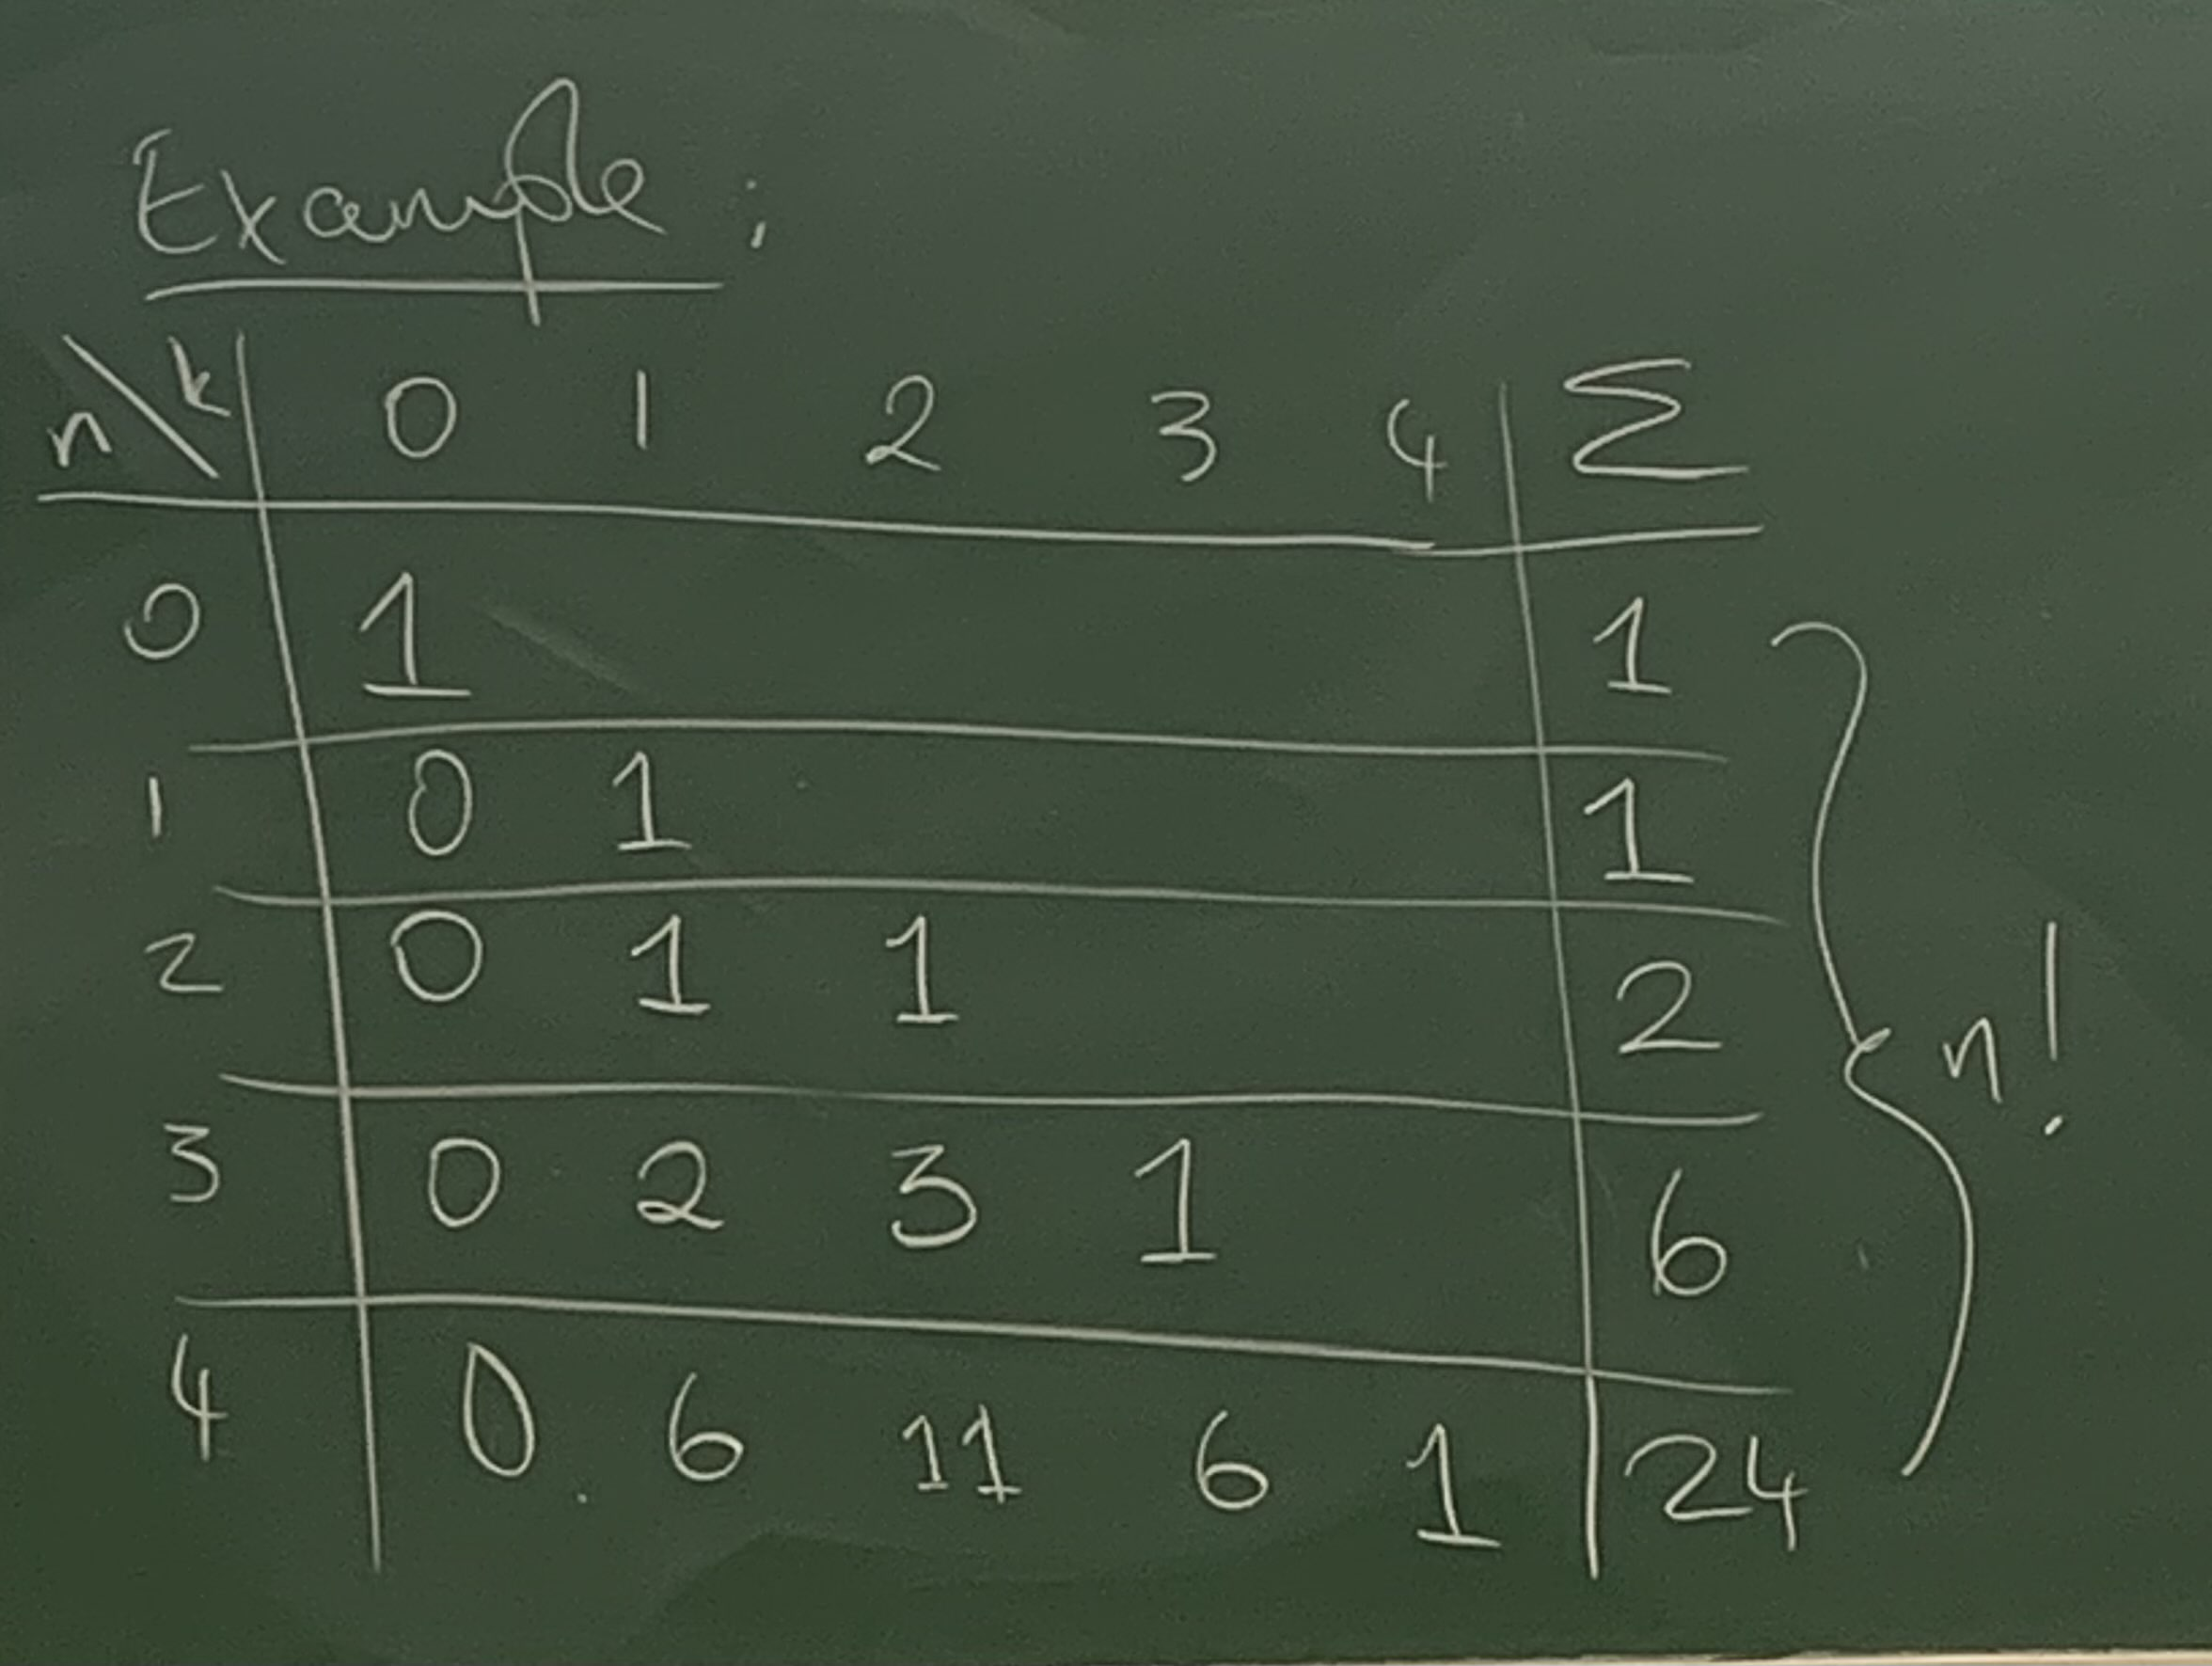
\includegraphics[width=0.6\textwidth]{./Figures/IMG_3936.jpg}
    \caption{table of \(s_{n,k}\)}
    \label{fig:table of Stirling number of first kind}
\end{figure}

\begin{corollary}
    \(\forall n\), we have 
    \[
        \sum_{k=0}^n s_{n,k} = n!. 
    \] 
\end{corollary}
\begin{proof}
    The number of permutations are \(n!\), and every permutation consists of \(i\) cycles where \(1 \le i \le n\), and then apply the sum rule.   
\end{proof}

\begin{notation}
    Given \(x \in F\), and \(k \in \mathbb{N} \cup \left\{ 0 \right\} \), we have 
    \begin{itemize}
        \item \(x^{\underline{k}} = x(x-1)\dots (x-(k-1))\) 
        \item \(x^{\overline{k} } = x(x+1)\dots (x+(k-1)) = (x+k-1)^{\underline{k}}\).  
    \end{itemize}
\end{notation}

\begin{proposition} \label{prop: a summation formula for first kind of striling number}
    For all \(x \in F\), \(n \in \mathbb{N} \cup \left\{ 0 \right\} \), 
    \[
        x^{\overline{n} }= \sum_{k=0}^n s_{n,k} x^k. 
    \]  
\end{proposition}
\begin{proof}
    Induction on \(n\). We know it is true for \(n=0,1\). Note that 
    \begin{align*}
        x^{\overline{n} } &= x^{\overline{n-1}}(x+n-1) \\
        &= (x+n-1) \sum_{k=0}^{n-1} s_{n-1,k} x^k \\
        &= x \sum_{k=0}^{n-1}s_{n-1,k} x^k + (n-1) \sum_{k=0}^{n-1} s_{n-1, k} x^k \\
        &= \sum_{k=0}^{n-1} s_{n-1,k} x^{k+1} + \sum_{k=0}^{n-1}(n-1)s_{n-1,k}x^k \\
        &= \sum_{k=1}^n s_{n-1, k-1} x^{k} + \sum_{k=0}^{n-1}(n-1)s_{n-1,k}x^k \\
        &= \sum_{k=0}^n \left( s_{n-1,k-1}+(n-1)s_{n-1,k} \right) x^k \\
        &= \sum_{k=0}^n s_{n,k} x^k.          
    \end{align*} 
\end{proof}

\begin{corollary}
    \[
         x^{\underline{n}} = \sum_{k=0}^n \underbrace{(-1)^{n-k} s_{n,k}}_{\substack{\text{signed Stirling numbers} \\ \text{of the first kind}}}x^k .
    \]
\end{corollary}
\begin{proof}
    \begin{align*}
        x^{\underline{n}} &= x(x-1)\dots (x-(n-1)) \\
        &= (-1)^n (-x)(-x+1)\dots (-x+(n-1)) \\
        &=(-1)^n (-x)^{\overline{n} } \\
        &= (-1)^n \sum_{k=0}^n s_{n,k}(-x)^k \\
        &= \sum_{k=0}^n (-1)^{n-k} s_{n,k} x^k. 
    \end{align*}
\end{proof}